\documentclass[journal,12pt,onecolumn]{IEEEtran}
\usepackage{graphicx, float}
\graphicspath{{Figs/}}
\usepackage{multicol}
\usepackage{parskip}
\usepackage{titlesec}
\usepackage{color}
\usepackage{enumitem}
\usepackage{amsmath,amssymb,amsfonts,amsthm}
\usepackage{array}
\usepackage{booktabs}
\usepackage[table]{xcolor}
\usepackage{longtable}
\usepackage{gensymb}
\usepackage{cite}
\usepackage{algorithmic}
\usepackage{textcomp}
\usepackage{txfonts}
\usepackage{listings}
\usepackage{mathtools}
\usepackage{comment}
\usepackage{tkz-euclide}
\usepackage[breaklinks=true]{hyperref}
\usepackage{gvv}
\usepackage[latin1]{inputenc}
\usetikzlibrary{arrows.meta, positioning}
\usepackage{xparse}
\usepackage{calc}
\usepackage{multirow}
\usepackage{hhline}
\usepackage{ifthen}
\usepackage{lscape}
\usepackage{tabularx}
\usepackage{circuitikz}
\usepackage{tikz}
\newtheorem{problem}{Problem}
\newtheorem{theorem}{Theorem}[section]
\newtheorem{proposition}{Proposition}[section]
\newtheorem{lemma}{Lemma}[section]
\newtheorem{corollary}[theorem]{Corollary}
\newtheorem{example}{Example}[section]
\newtheorem{definition}[problem]{Definition}
\newcommand{\BEQA}{\begin{eqnarray}}
\newcommand{\EEQA}{\end{eqnarray}}
\theoremstyle{remark}
\usepackage{pgfplots}
\pgfplotsset{compat=1.18}

\usepackage{tikz}

\title{GATE AG 2023}
\author{ai25btech11028 R.Manohar}
\begin{document}
\maketitle

\subsection{Q.1-Q.5 Carry ONE mark Each}
\begin{enumerate}

\item ''You are delaying the completion of the task. Send \_\_\_\_\_ contributions at the earliest.''
\begin{multicols}{4}
\begin{enumerate}
    \item you are
    \item your
    \item you're
    \item yore
\end{enumerate}
\end{multicols}
\hfill{(GATE AG 2023)}

\item References : \_\_\_\_\_ : : Guidelines : Implement (By word meaning)
\begin{multicols}{4}
\begin{enumerate}
    \item Sight
    \item Site
    \item Cite
    \item Plagiarise
\end{enumerate}
\end{multicols}
\hfill{(GATE AG 2023)}

\item In the given figure, $PQRS$ is a parallelogram with $PS=7$ cm, $PT=4$ cm and $PV=5$ cm. What is the length of $RS$ in cm? (Diagram is representative.)
\begin{figure}[H]
    \centering
    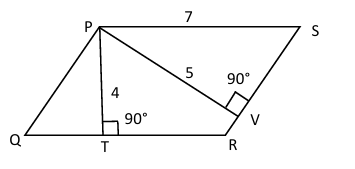
\includegraphics[]{figs/Q.3.png}
    \caption{}
    \label{fig:1}
\end{figure}
\begin{multicols}{4}
\begin{enumerate}
    \item $\tfrac{20}{7}$
    \item $\tfrac{28}{5}$
    \item $\tfrac{9}{2}$
    \item $\tfrac{35}{4}$
\end{enumerate}
\end{multicols}
\hfill{(GATE AG 2023)}

\item In 2022, June Huh was awarded the Fields medal, the highest prize in Mathematics. When he was younger, he was also a poet. He did not win any medals in the International Mathematics Olympiads. He dropped out of college. 
Based only on this information, which can be inferred with \emph{certainty}?
\begin{enumerate}
    \item Every Fields medalist has won a medal in an International Mathematics Olympiad.
    \item Everyone who has dropped out of college has won the Fields medal.
    \item All Fields medalists are part-time poets.
    \item Some Fields medalists have dropped out of college.
\end{enumerate}
\hfill{(GATE AG 2023)}

\item A line of symmetry divides a figure into two parts that are mirror images. In the given figure with 16 unit squares, in addition to the three black squares, what is the minimum number of squares that must be coloured black so that both $PQ$ and $MN$ are lines of symmetry?
\begin{figure}[H]
    \centering
    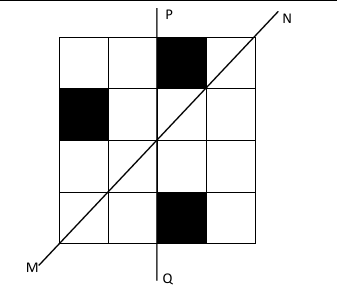
\includegraphics[]{figs/Q.5.png}
    \caption{}
    \label{fig:2}
\end{figure}
\begin{multicols}{4}
\begin{enumerate}
    \item 3
    \item 4
    \item 5
    \item 6
\end{enumerate}
\end{multicols}
\hfill{(GATE AG 2023)}

\item Human beings are among many creatures in an imagined world. Some creatures are cruel. If the statement ``Some human beings are not cruel creatures'' is FALSE, then which statements can be inferred with certainty?\\ 
(i) All human beings are cruel.\\ 
(ii) Some human beings are cruel. \\
(iii) Some cruel creatures are humans. \\
(iv) No human beings are cruel.
\begin{multicols}{2}
\begin{enumerate}
    \item only (i)
    \item only (iii) and (iv)
    \item only (i) and (ii)
    \item (i), (ii) and (iii)
\end{enumerate}
\end{multicols}
\hfill{(GATE AG 2023)}

\item To construct a wall, sand and cement are mixed in the ratio $3:1$. The cost ratio of sand and cement is $1:2$. If the total cost is 1000 rupees, what is the cost (in rupees) of cement?
\begin{multicols}{4}
\begin{enumerate}
    \item 400
    \item 600
    \item 800
    \item 200
\end{enumerate}
\end{multicols}
\hfill{(GATE AG 2023)}

\item The World Bank has declared it will not offer new financing to Sri Lanka until it has an adequate macroeconomic policy. It has repurposed resources from existing loans to help with essential items. 
Based only on this passage, which one can be inferred with certainty?
\begin{enumerate}
    \item According to the World Bank, the root cause of Sri Lanka's crisis is lack of foreign exchange.
    \item The World Bank has stated it will advise Sri Lanka on tackling the root causes.
    \item According to the World Bank, Sri Lanka does not yet have an adequate macroeconomic policy framework.
    \item The World Bank will provide Sri Lanka with additional funds for essentials.
\end{enumerate}
\hfill{(GATE AG 2023)}

\item The coefficient of $x^4$ in $(x-1)^3(x-2)^3$ is equal to \_\_\_\_\_.
\begin{multicols}{4}
\begin{enumerate}
    \item 33
    \item $-3$
    \item 30
    \item 21
\end{enumerate}
\end{multicols}
\hfill{(GATE AG 2023)}

\item Which one of the following shapes can be used to tile the plane (cover completely without gaps/overlap)?
\begin{multicols}{4}
\begin{enumerate}
    \item circle
    \item regular octagon
    \item regular pentagon
    \item rhombus
\end{enumerate}
\end{multicols}
\hfill{(GATE AG 2023)}

\item If $A$ and $B$ are $3\times 3$ matrices such that $|A|=-1$, $|B|=3$, then $|3AB|$ equals
\begin{multicols}{4}
\begin{enumerate}
    \item $-81$
    \item $-27$
    \item $-9$
    \item $81$
\end{enumerate}
\end{multicols}
\hfill{(GATE AG 2023)}

\item 
\begin{align*}
\lim\limits_{x \to 0} \frac{\sqrt{1+x}-1}{x}
\end{align*}
equals
\begin{multicols}{4}
\begin{enumerate}
    \item 0
    \item $\tfrac{1}{2}$
    \item 1
    \item 2
\end{enumerate}
\end{multicols}
\hfill{(GATE AG 2023)}

\item The value of
\begin{align*}
I = \int_0^{\pi/2} \frac{(\sin x + \cos x)^2}{\sqrt{1+\sin 2x}} \, dx
\end{align*}
is
\begin{enumerate}
    \item 0
    \item 1
    \item 2
    \item 3
\end{enumerate}
\hfill{(GATE AG 2023)}

\item 
\begin{align*}
y = ae^{mx} + be^{-mx} 
\end{align*}
is the solution of which differential equation?
\begin{enumerate}
    \item $\tfrac{dy}{dx} - my = 0$
    \item $\tfrac{dy}{dx} + my = 0$
    \item $\tfrac{d^2y}{dx^2} + m^2 y = 0$
    \item $\tfrac{d^2y}{dx^2} - m^2 y = 0$
\end{enumerate}
\hfill{(GATE AG 2023)}

\item In rotary tiller, the total energy requirement for carrying out tillage will decrease if
\begin{enumerate}
    \item the bite length is increased
    \item the bite length is decreased
    \item the cone index of soil is higher
    \item forward speed of the machine is reduced
\end{enumerate}
\hfill{(GATE AG 2023)}

\item The effectiveness of the turbocharger of a diesel engine increases when
\begin{enumerate}
    \item the ambient temperature increases
    \item the pressure ratio across the compressor decreases
    \item the load on the engine increases
    \item the displacement volume of the engine decreases
\end{enumerate}
\hfill{(GATE AG 2023)}

\item In a thresher, the cylinder separation efficiency can be improved by increasing
\begin{enumerate}
    \item cylinder diameter
    \item cylinder speed
    \item cylinder-concave clearance
    \item feed rate
\end{enumerate}
\hfill{(GATE AG 2023)}

\item In a 4-stroke single cylinder diesel engine, the inlet valve opens at 10° before TDC and closes at 40° after BDC. The exhaust valve opens at 25° before BDC and closes at 15° after TDC. The percentage of time for which both the valves remain closed in one cycle of the engine is
\begin{enumerate}
    \item 32.29
    \item 40.97
    \item 46.53
    \item 75.01
\end{enumerate}
\hfill{(GATE AG 2023)}

\item The torque available at maximum power developed by the tractor is 150 N m. If the reserve torque is 20\%, the peak torque that can be developed by the tractor in N m is
\begin{enumerate}
    \item 100
    \item 120
    \item 180
    \item 210
\end{enumerate}
\hfill{(GATE AG 2023)}

\item The statement which is not correct for the porous medium is
\begin{enumerate}
    \item Seepage velocity is always greater than the Darcy's velocity
    \item Darcy's velocity is not exclusively controlled by soil porosity
    \item Seepage velocity increases with increasing surface ponding of water
    \item Darcy's velocity in unsaturated soil is always greater than that in saturated soil
\end{enumerate}
\hfill{(GATE AG 2023)}

\item A sprinkler irrigation system has been designed for a crop with the water application rate of 1.17 cm h$^{-1}$ and sprinkler discharge of 1.3 L s$^{-1}$. The coefficient of discharge and uniformity coefficient are 0.9 and 0.8, respectively. If the sprinkler spacing along the lateral is 20 m, the lateral spacing in m is
\begin{enumerate}
    \item 14.4
    \item 16.0
    \item 18.0
    \item 20.0
\end{enumerate}
\hfill{(GATE AG 2023)}

\item The average discharge, operating pressure and emitter constant of a drip emitter are 4 L h$^{-1}$, 110 kPa and 0.3, respectively. The type of emitter is
\begin{enumerate}
    \item orifice
    \item long path
    \item pressure compensating
    \item disc
\end{enumerate}
\hfill{(GATE AG 2023)}

\item If the departure and latitude of a line are 70 m and -130 m, respectively, then the whole circle bearing of the line in degrees is
\begin{enumerate}
    \item 28
    \item 62
    \item 152
    \item 208
\end{enumerate}
\hfill{(GATE AG 2023)}

\item Match the Columns:

\begin{center}
\begin{tabular}{ll}
\textbf{I} & \textbf{II} \\
1. Tensiometer & a. Consumptive use \\
2. Piezometer & b. Bernoulli's equation \\
3. Lysimeter & c. Soil moisture \\
4. Elbow meter & d. Hydrostatic pressure \\
5. Pitot tube & e. Volumetric flow rate \\
\end{tabular}
\end{center}

\begin{enumerate}
    \item 1-c, 2-b, 3-a, 4-e, 5-d
    \item 1-c, 2-d, 3-a, 4-e, 5-b
    \item 1-d, 2-c, 3-e, 4-a, 5-b
    \item 1-c, 2-d, 3-a, 4-b, 5-e
\end{enumerate}
\hfill{(GATE AG 2023)}

\item The information needed for estimating the design flood using Rational formula is
\begin{enumerate}
    \item cumulative infiltration
    \item antecedent moisture condition of soil
    \item shape factor of the catchment
    \item time of concentration of the catchment
\end{enumerate}
\hfill{(GATE AG 2023)}

\item The microbial death kinetics for a food suspension follows the equation:
    \begin{align*}
    \log \frac{N_{0}}{N} = 1 + \frac{t-t_{1}}{D} 
    \end{align*}
    where $N_{0}$ = initial microbial load, $N$ = microbial load after time $t$, $t_{1}$ = lag time and $D$ = decimal reduction time.
    The correct statement for this equation is
    \begin{enumerate}
        \item the time required to reduce 10\% of the initial population is lag time.
        \item the time required to reduce the initial 90\% of population is lag time
        \item time required to kill the first 90\% population is lower than $D$ value at the same temperature
        \item lag time approaches $D$ value as $N_{0}$ becomes smaller and temperature decreases.
    \end{enumerate}
\hfill{(GATE AG 2023)}

    \item If the diameter of fat globule in a cream separator is reduced to half and the rotational speed of the centrifuge increased to three times, the terminal settling velocity of fat globule is
    \begin{enumerate}
    \begin{multicols}{2}
        \item decreased to 0.44 times
        \item increased to 0.44 times
        \item decreased to 2.25 times
        \item increased to 2.25 times
        \end{multicols}
    \end{enumerate}
\hfill{(GATE AG 2023)}

    \item The log mean temperature difference (LMTD) correction factor is not required during heat transfer rate calculation in
    \begin{enumerate}
        \item plate heat exchanger
        \item 1 shell pass and 1 tube pass heat exchanger
        \item 1 shell pass and 2 tube pass heat exchanger
        \item 2 shell pass and 4 tube pass heat exchanger
    \end{enumerate}
\hfill{(GATE AG 2023)}

    \item Identify the dimensionless parameter(s) from the following:
    \begin{enumerate}
    \begin{multicols}{4}
        \item Cone index
        \item Puddling index
        \item Performance index
        \item Reel index
        \end{multicols}
    \end{enumerate}
\hfill{(GATE AG 2023)}

    \item The probability that a storm event with a return period of 20 years will occur once in 5-year period is \_\_\_\_\_\_\_\_\_ (rounded off to 2 decimal places).
\hfill{(GATE AG 2023)}

    \item Considering declining balance method, the constant rate of depreciation at which the value of the tractor will come down to 50\% of its purchase price at the end of $4^{th}$ year in per cent is \_\_\_\_\_\_\_\_\_\_\_\_(rounded off to 2 decimal places).
\hfill{(GATE AG 2023)}

    \item A trapezoidal grassed waterway with side slope (H:V) of 1:1 carries a design discharge of 1 m$^{3}$ s$^{-1}$. The bed slope and Manning's roughness coefficient of this channel are 1\% and 0.04, respectively. The design depth of the best hydraulic trapezoidal grassed waterway section in m is \_\_\_\_\_\_\_\_\_\_\_\_\_ (rounded off to 2 decimal places).
\hfill{(GATE AG 2023)}

    \item The minimum fluidization height of 1.20 m is maintained during fluidized bed drying of carrots. The bed diameter of the fluidized bed dryer is 0.6 m. If mass and solid density of carrots are 250 kg and 1040 kg m$^{-3}$, respectively, then the porosity of the bed at the minimum fluidization condition is \_\_\_\_\_\_\_\_\_\_ (rounded off to 3 decimal places, Consider $\pi = 3.14$).
\hfill{(GATE AG 2023)}

    \item The lighter liquid layer and the interphase layer in a basket centrifuge, rotating at a speed of 1000 rpm, are 0.1025 m and 0.105 m away from the center, respectively. Considering the densities of lighter and heavier liquids as 920 kg m$^{-3}$ and 1015 kg m$^{-3}$, the differential pressure in horizontal direction required to maintain the interphase layer in kPa is \_\_\_\_\_\_\_\_\_\_\_\_\_\_\_\_\_\_\_\_\_\_\_ (rounded off to 3 decimal places, Consider $\pi = 3.14$).
\hfill{(GATE AG 2023)}

    \item The upstream and downstream pressures in a homogenizer during homogenization of milk are maintained at 250 bar and 10 bar, respectively. If density of milk is 1030 kg m$^{-3}$, then the velocity at which milk comes out of the homogenizing valve in m s$^{-1}$ is \_\_\_\_\_\_\_\_\_\_\_\_\_ (rounded off to 3 decimal places).
    \hfill{(GATE AG 2023)}

    \item If $A = \myvec{1 & 2 \\ -1 & 1}$, $B = \myvec{a & 1 \\ b & -1}$ and $(A+B)^{2} = A^{2} + B^{2}$, then the values of $a$ and $b$ are:
    \begin{multicols}{2}
    \begin{enumerate}
        \item $a = 4, b = 1$
        \item $a = 1, b = 4$
        \item $a = 0, b = 4$
        \item $a = 2, b = 4$
    \end{enumerate}
    \end{multicols}
\hfill{(GATE AG 2023)}

    \item A vector $\vec{P} = 5\hat{i} - 10\hat{j} + 8\hat{k}$ is passing through the origin of a 3-D frame. Considering the tendency of rotation in the counter clockwise direction as positive, the moment about a point A: (3, 4, 8) is
    \begin{multicols}{2}
    \begin{enumerate}
        \item $-16\hat{i} + 112\hat{j} + 50\hat{k}$
        \item $112\hat{i} + 16\hat{j} - 50\hat{k}$
        \item $50\hat{i} - 112\hat{j} + 16\hat{k}$
        \item $-112\hat{i} - 16\hat{j} + 50\hat{k}$
    \end{enumerate}
    \end{multicols}
\hfill{(GATE AG 2023)}

    \item A vertical disc plough with 5 discs is operated at a depth of 0.15 m. The disc angle and disc diameter are $40^{0}$ and 0.6 m, respectively. If overlap between two consecutive discs is 0.12 m at 0.15 m depth of cut, the total width of cut at the specified depth in m is
    \begin{multicols}{4}
    \begin{enumerate}
        \item 1.19
        \item 1.55
        \item 2.11
        \item 2.36
    \end{enumerate}
    \end{multicols}
\hfill{(GATE AG 2023)}

    \item In a 9$\times$20 cm fluted roller type seed drill, each fluted roller is discharging 4.25 g of seed per revolution of fluted roller shaft. The fluted roller shaft rotates once for two complete rotation of the ground drive wheel of the seed drill. The rolling diameter of the ground drive wheel is 0.35 m. Considering no skid of the ground drive wheel, the seed rate in kg ha$^{-1}$ is
    \begin{multicols}{4}
    \begin{enumerate}
        \item 96.62
        \item 141.55
        \item 187.35
        \item 386.42
    \end{enumerate}
    \end{multicols}
\hfill{(GATE AG 2023)}

    \item A field sprayer with 12 nozzles fitted to the boom at a spacing of 0.5 m is used for spraying at a height of 0.75 m from the ground. The angle of spraying is $75^{o}$. If the height of spraying is reduced to 0.6 m, the change in swath in m is
    \begin{multicols}{4}
    \begin{enumerate}
        \item 0.23
        \item 0.48
        \item 0.65
        \item 0.91
    \end{enumerate}
    \end{multicols}
\hfill{(GATE AG 2023)}

    \item The ordinates of a 6-hour S-hydrograph of a catchment are given in Table below. The catchment has phi-index of 0.25 cm h$^{-1}$ and baseflow of 10.5 m$^{3}$ s$^{-1}$. The peak of the flood hydrograph generated from this catchment due to a storm of 45 mm received during the first 6 h in m$^{3}$ s$^{-1}$ is
    \begin{tabular}{|l|c|c|c|c|c|c|c|c|c|}
        \hline
        Time (h) & 0 & 6 & 12 & 18 & 24 & 30 & 36 & 42 & 48 \\
        \hline
        Ordinate (m$^{3}$ s$^{-1}$) & 0 & 30 & 90 & 180 & 252 & 306 & 342 & 360 & 360 \\
        \hline
    \end{tabular}
    \begin{multicols}{4}
    \begin{enumerate}
        \item 259.5
        \item 270.0
        \item 280.5
        \item 349.5
    \end{enumerate}
    \end{multicols}
\hfill{(GATE AG 2023)}

    \item It is planned to provide irrigation in a crop field having field capacity and permanent wilting point of the soil as 0.21 cm$^{3}$ cm$^{-3}$ and 0.09 cm$^{3}$ cm$^{-3}$, respectively. The crop root zone depth is 0.90 m. The growing period of this crop is $1^{st}$ January to $31^{st}$ March, during which the observed reference evapotranspiration (ET$_{0}$), effective rainfall (P$_{e}$) and crop coefficients (K$_{c}$) are listed below. Considering management allowable deficit (MAD) for this crop as 50\%, the average irrigation interval during the growing period in days is
    \begin{tabular}{|l|c|c|c|}
        \hline
        Month & January & February & March \\
        \hline
        ET$_{0}$ (mm day$^{-1}$) & 11 & 12 & 14 \\
        \hline
        P$_{e}$ (mm month$^{-1}$) & 8 & 25 & 27 \\
        \hline
        K$_{c}$ & 0.80 & 1.10 & 1.15 \\
        \hline
    \end{tabular}
    \begin{multicols}{4}
    \begin{enumerate}
        \item 4
        \item 6
        \item 8
        \item 11
    \end{enumerate}
    \end{multicols}
\hfill{(GATE AG 2023)}

    \item The infiltration capacity of a basin is described by the Horton's equation,
    \begin{align*}
    I = 2 + e^{-3t},
    \end{align*}
    where $I$ is in cm h$^{-1}$ and the duration, $t$ is in hours. If the duration of the storm event is 2 hours, the depth of the infiltration in the last 1 hour of the storm event in mm is
    \begin{multicols}{4}
    \begin{enumerate}
        \item 5
        \item 10
        \item 20
        \item 25
    \end{enumerate}
    \end{multicols}
\hfill{(GATE AG 2023)}

    \item In a juice filtration process, solid concentration per m$^{3}$ of filtrate is 0.2 kg. During filtration of 12.49 m$^{3}$ of juice, 0.02 m thick cake (porosity of 0.32) is deposited. If 2.5 kg of solid is collected in 180 s, the pressure drop across the cake in kPa is
    [Absolute viscosity of juice is $2.12 \times 10^{-3}$ kg m$^{-1}$ s$^{-1}$, and specific cake resistance is $1.2 \times 10^{9}$ m kg$^{-1}$]
    \begin{multicols}{4}
    \begin{enumerate}
        \item 0.18
        \item 1.81
        \item 18.06
        \item 180.60
    \end{enumerate}
    \end{multicols}
\hfill{(GATE AG 2023)}

    \item Cheese is packed in a bilayer plastic package made up of low density polyethylene (LDPE) and polyethylene terephthalate (PET). The thickness of LDPE and PET in the package are 1.5 mm and 1.3 mm, respectively. The surface area of the plastic package is 6.25 cm$^{2}$. The partial pressure difference of oxygen across the package wall is 0.30 atm. The permeability coefficient of oxygen in LDPE and PET are $4.18 \times 10^{-8}$ cm cm$^{2}$ s$^{-1}$ atm$^{-1}$ and $1.67 \times 10^{-10}$ cm cm$^{2}$ s$^{-1}$ atm$^{-1}$, respectively. If the food gets spoiled when it absorbs 0.025 ml of oxygen, then the shelf life of food in days is
    \begin{multicols}{4}
    \begin{enumerate}
        \item 121
        \item 103
        \item 73
        \item 61
    \end{enumerate}
    \end{multicols}
\hfill{(GATE AG 2023)}

    \item The rotor shaft of an ice cream freezer consists of 3 scraper blades. The temperature difference between the ice cream mix and the refrigerant during freezing of ice cream is 30$^{o}$C. Density and latent heat of fusion of ice are 917 kg m$^{-3}$ and 335 kJ kg$^{-1}$, respectively. The overall heat transfer coefficient is 2000 kJ m$^{-2}$ h$^{-1}$ $^{o}$C$^{-1}$. If the maximum thickness of ice formed before being scraped off is 10 $\mu$m, the minimum speed of the scraper shaft in rpm is
    \begin{multicols}{4}
    \begin{enumerate}
        \item 88
        \item 109
        \item 121
        \item 149
    \end{enumerate}
    \end{multicols}
\hfill{(GATE AG 2023)}

    \item The percentage absolute humidity of air becomes equal to the percentage relative humidity, when
    \begin{enumerate}
        \item absolute humidity of air is equal to relative humidity
        \item saturated humidity of air is equal to relative humidity
        \item air is almost or completely dry
        \item air is almost or completely saturated
    \end{enumerate}
\hfill{(GATE AG 2023)}

    \item Dimensionless numbers play an important role in correlating transfer coefficients during forced convection. In relation to the dimensionless numbers, the correct statement(s) is/are
    \begin{enumerate}
        \item Prandtl number in heat transfer is analogous to Schmidt number in mass transfer
        \item Small value of Prandtl number signifies lower thermal diffusion as compared to momentum diffusion
        \item Prandtl number is the ratio of momentum diffusivity to the thermal diffusivity of the fluid
        \item Lewis number is the product of Schmidt number and Prandtl number
    \end{enumerate}
\hfill{(GATE AG 2023)}

    \item In a locality 'A', the probability of a convective storm event is 0.7 with a density function, $f_{X_{1}}(x_{1}) = e^{-x_{1}}, x_{1} > 0$. The probability of tropical cyclone-induced storm in the same location is given by the density function $f_{X_{2}}(x_{2}) = 2e^{-2x_{2}}, x_{2} > 0$. The probability of occurring more than 1 unit of storm event is \_\_\_\_\_\_\_\_\_\_\_ (rounded off to 2 decimal places).
\hfill{(GATE AG 2023)}

    \item Given that $\frac{dy}{dx} = 2x+y$ and $y=1$, when $x=0$. Using Runge-Kutta fourth order method, the value of $y$ at $x=0.2$ is \_\_\_\_\_\_\_\_\_\_\_\_ (rounded off to 3 decimal places).
\hfill{(GATE AG 2023)}

\item A power operated chaff cutter with a mean cutting radius of 0.25 m is fitted with two cutting knives and is rotating at 300 rpm. Thirty maize stalks with a mean diameter of 12 mm are fed through the throat at a time. The dynamic shear strength of the stalk is 0.05 N mm$^{-2}$. The mass and radius of gyration of the flywheel (including knives) are 40 kg and 0.27 m, respectively. The total shaft power requirement in kW is \_\_\_\_\_\_\_\_\_\_ (rounded off to 2 decimal places).
\hfill{(GATE AG 2023)}

    \item A two-wheel drive tractor with a total weight of 24 kN has a static weight distribution of 30\% and 70\% at the front and rear axles, respectively. When the tractor is operated on a level ground of pure sand, the maximum tractive force developed is 13 kN. If external weight of 1.5 kN is added to the rear axle, neglecting weight transfer, the change in maximum tractive force in kN is \_\_\_\_\_\_\_\_\_\_\_\_(rounded off to 2 decimal places).
    \hfill{(GATE AG 2023)}

    \item A 4-stroke diesel engine can be operated with either diesel (heating value 45 MJ kg$^{-1}$) or biodiesel blend, B20 (heating value 42.1 MJ kg$^{-1}$). The brake specific fuel consumption of the engine when operated with diesel and B20 is 260 g kW$^{-1}$ h$^{-1}$ and 310 g kW$^{-1}$ h$^{-1}$, respectively. For developing a brake power of 20 kW, the change in brake thermal efficiency of the engine when B20 is used in place of diesel is \_\_\_\_\_\_\_\_\_\_\_ (rounded off to 2 decimal places).
    \hfill{(GATE AG 2023)}

    \item A solar photovoltaic system is used to generate power from total solar radiations varying from 400 to 750 W m$^{-2}$. The maximum conversion efficiency of solar photovoltaic system is 14\%. The open circuit voltage, short circuit current and fill factor of solar cells are 21.6 V, 3.22 A and 0.72, respectively. To generate maximum power, the minimum cell area required in m$^{2}$ is \_\_\_\_\_\_\_\_\_\_\_ (rounded off to 3 decimal places).
\hfill{(GATE AG 2023)}

    \item A single disc clutch is used to transmit 10 kW power at 1400 rpm. The axial pressure exerted on the contact surface is 0.07 N mm$^{-2}$ and the coefficient of friction is 0.25. Considering the ratio of diameter to face width of the clutch lining as 8 and assuming uniform wear theory, the required face width of friction lining in mm is \_\_\_\_\_\_\_\_\_\_\_\_\_\_ (rounded off to 2 decimal places).
\hfill{(GATE AG 2023)}

    \item In a tractor seat system, the chassis frequency and seat suspension damping rate are 20 rad s$^{-1}$ and 400 N m$^{-1}$ s, respectively. The critical damping rate of tractor seat system is 1600 N m$^{-1}$ s. If the combined mass of the seat and operator is 80 kg, the transmissibility of vibration is \_\_\_\_\_\_\_\_\_\_\_\_\_\_ (rounded off to 2 decimal places).
\hfill{(GATE AG 2023)}

    \item Two cylindrical reservoirs 'A' and 'B' are connected by a 30 m long pipe of 250 mm internal diameter as shown in Figure below. The Darcy-Weisbach friction factor for the pipe is 0.025. Initially the reservoir 'A' was full at the indicated level and reservoir 'B' was empty. If the entrance and exit losses in this pipe are neglected, the time required to empty the reservoir 'A' in hour is \_\_\_\_\_\_\_\_\_\_\_\_\_ (rounded off to 3 decimal places).
    Consider $\pi = 3.14$ and acceleration due to gravity, $g = 9.81$ m s$^{-2}$.

\begin{figure}[H]
    \centering
    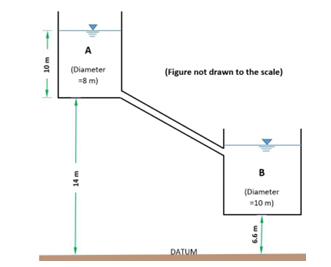
\includegraphics[]{figs/Q.57.png}
    \caption{}
    \label{fig:3}
\end{figure}
\hfill{(GATE AG 2023)}

    \item A homogeneous anisotropic earthen dam of height 52 m with a free board of 2 m is constructed on an impermeable foundation. The horizontal and vertical hydraulic conductivities of soil used for the construction of the dam are $4.5 \times 10^{-8}$ m s$^{-1}$ and $2.0 \times 10^{-8}$ m s$^{-1}$, respectively. There are 6 flow channels and 25 equipotential drops in a square flownet drawn in the transformed dam section. If the downstream dam side is dry, the quantity of seepage per unit length through the dam in m$^{3}$ day$^{-1}$ m$^{-1}$ is \_\_\_\_\_\_\_\_\_\_\_\_\_ (rounded off to 3 decimal places).
\hfill{(GATE AG 2023)}

    \item A salt affected crop field is to be leached with irrigation water having salt concentration of 3.5 meq L$^{-1}$. Salt concentration in the saturation extract of soil is 15.2 meq L$^{-1}$. Leaching efficiency of the field is 55\%. In the month of March, the observed reference evapotranspiration and effective rainfall in this area are 150 mm and 75 mm, respectively. If the average crop coefficient in this month is 1.05, the leaching requirement for the entire month in mm is \_\_\_\_\_\_\_\_\_\_\_\_\_\_\_ (rounded off to 2 decimal places).
\hfill{(GATE AG 2023)}

    \item A 10 m long concrete pipe is required to carry a peak discharge of 1.0 m$^{3}$ s$^{-1}$ in a drop inlet spillway with a head of 4 m. The entrance loss coefficient is 0.5 and the friction loss coefficient is 0.02. Consider acceleration due to gravity = 9.81 m s$^{-2}$. The neutral slope of the water level in per cent is \_\_\_\_\_\_\_\_\_\_\_\_\_\_\_\_\_\_\_ (rounded off to 2 decimal places).
\hfill{(GATE AG 2023)}

    \item Discharge from a centrifugal pump operating at 1000 rpm with a total head of 30 m is 300 L min$^{-1}$. The pump efficiency is 65\%. If speed of the pump is increased to 1200 rpm, the power required to operate the pump in kW is \_\_\_\_\_\_\_\_\_\_\_\_\_\_\_\_ (rounded off to 2 decimal places).
    Consider acceleration due to gravity = 9.81 m s$^{-2}$.
\hfill{(GATE AG 2023)}

    \item A 0.30 m diameter well penetrates an unconfined aquifer with a saturated depth of 40 m. After 8 hours of pumping at a steady rate of 0.03 m$^{3}$ s$^{-1}$, the drawdown in two observation wells located at 20 m and 50 m away from the pumping well are found to be 3 m and 2 m, respectively. The drawdown in the pumping well in m is \_\_\_\_\_\_\_\_\_\_\_\_\_\_\_\_\_\_ (rounded off to 1 decimal place, Consider $\pi = 3.14$).
    \hfill{(GATE AG 2023)}

    \item The apparent wall shear stress in a 0.6 m long pipe carrying refined oil is 12.5 Pa. If the pressure drop along the length is 300 Pa and flow rate is 0.25 m$^{3}$ s$^{-1}$, the absolute viscosity of oil in 10$^{-3}$ Pa s is \_\_\_\_\_\_\_\_\_\_\_\_\_\_\_\_\_\_ (rounded off to 3 decimal places).
\hfill{(GATE AG 2023)}

    \item The carrot slices (water activity = 0.89) are to be preserved using osmo-dehydration. Addition of salt (NaCl) to 20\% sucrose solution (water activity = 0.987) reduces the water activity to 0.85. Percentage of NaCl added to the solution is \_\_\_\_\_\_\_\_\_\_\_\_\_\_\_\_\_\_\_\_ (rounded off to 2 decimal places).
    Consider molecular mass of Sucrose = 342 and molecular mass of NaCl = 58.44
\hfill{(GATE AG 2023)}

    \item A copper ball and a steel ball having diameters $d_{1}$ and $d_{2}$, respectively, are initially at a uniform temperature of 200 $^{o}$C. Both the balls are exposed to the atmosphere at 30 $^{o}$C. If both the balls attain a temperature of 120 $^{o}$C after equal exposure duration, then the ratio of d$_{1}$ to d$_{2}$ is \_\_\_\_\_\_\_\_\_\_\_\_\_ (rounded off to 3 decimal places).
    Assume Biot Number to be less than 0.1. The thermo-physical properties of copper and steel are given below:

    
    \begin{tabular}{|l|c|c|c|}
        \hline
        Material & Density (kg m$^{-3}$) & Specific heat (J kg$^{-1}$ $^{o}$C$^{-1}$) & Thermal conductivity (W m$^{-1}$ $^{o}$C$^{-1}$) \\
        \hline
        Copper & 8950 & 383 & 386 \\
        \hline
        Steel & 7800 & 460 & 36 \\
        \hline
    \end{tabular}
    \hfill{(GATE AG 2023)}

\end{enumerate}
\end{document}